\chapter*{Konzeptentwurf}
\label{cha:Konzeptentwurf}
\begin{comment} % Aus Angabe:
Erstellung eines Konzept (Planung) mit geeigneter (kompakter) Dokumentation \newline
* Signalliste \\
* Statemachine \\
\end{comment}
Text Text Text...
\begin{table}[h!]
	\centering
	%\renewcommand{\arraystretch}{1.0} % Verringert den Zeilenabstand
	%\small
	\begin{tabular}{|l|l|l|l|}
		\hline
		\textbf{Name} & \textbf{Datentyp} & \textbf{Adresse} & \textbf{Kommentar}\\ \hline
		RED\_button\_released & Bool & \%I193.2 &  \\ \hline
		Green\_button\_pressed & Bool & \%I193.3 &  \\ \hline
		Red\_button\_LED\_ON & Bool & \%Q192.0 &  \\ \hline
		Green\_button\_LED\_ON & Bool & \%Q192.1 &  \\ \hline
	\end{tabular}
	\caption{Variablentabelle von AC2398}
	\label{tab:AC2398}
\end{table}
\begin{table}[h!]
	\centering
	\begin{tabular}{|l|l|l|l|}
		\hline
		\textbf{Name} & \textbf{Datentyp} & \textbf{Adresse} & \textbf{Kommentar} \\ \hline
		Output\_Param.Done & Bool & \%I6.0 & \\ \hline
		Output\_Param.Busy & Bool & \%I6.1 & \\ \hline
		Output\_Param.Error & Bool & \%I6.2 & \\ \hline
		Output\_Param.Status & Word & \%IW8 & \\ \hline
		Output\_Param.ExtStatus & DWord & \%ID10 & \\ \hline
		Output\_Param.RdValue & UInt & \%IW14 & \\ \hline
		Output\_Data.TagPresent & Bool & \%I92.0 & \\ \hline
		Output\_Data.Done & Bool & \%I92.1 & \\ \hline
		Output\_Data.Busy & Bool & \%I92.2 & \\ \hline
		Output\_Data.Error & Bool & \%I92.3 & \\ \hline
		Output\_Data.Status & Word & \%IW94 & \\ \hline
		Output\_Data.ExStatus & Word & \%IW96 & \\ \hline
		Input\_Param.Execute & Bool & \%Q0.0 & \\ \hline
		Input\_Param.Mode & UInt & \%QW2 & \\ \hline
		Input\_Param.SetValue & UInt & \%QW4 & \\ \hline
		Input\_Data.DT\_InAddr & UInt & \%QW16 & \\ \hline
		Input\_Data.DT\_OutAddr & UInt & \%QW18 & \\ \hline
		Input\_Data.Execute & Bool & \%Q20.0 & \\ \hline
		Input\_Data.Force & Bool & \%Q20.1 & \\ \hline
		Input\_Data.Mode & UInt & \%QW22 & \\ \hline
		Input\_Data.TagMemAddr & UInt & \%QW24 & \\ \hline
		Input\_Data.Length & UInt & \%QW26 & \\ \hline
		Input\_Data.WrData & Array[0..31] of UInt & \%Q28.0 & \\ \hline
		Input\_Data.RdData & Array[0..31] of UInt & \%Q60.0 & \\ \hline
	\end{tabular}
	\caption{Variablentabelle von DTI515}
	\label{tab:DTI515}
\end{table}
\newpage
\begin{figure}[h!]
	\centering
	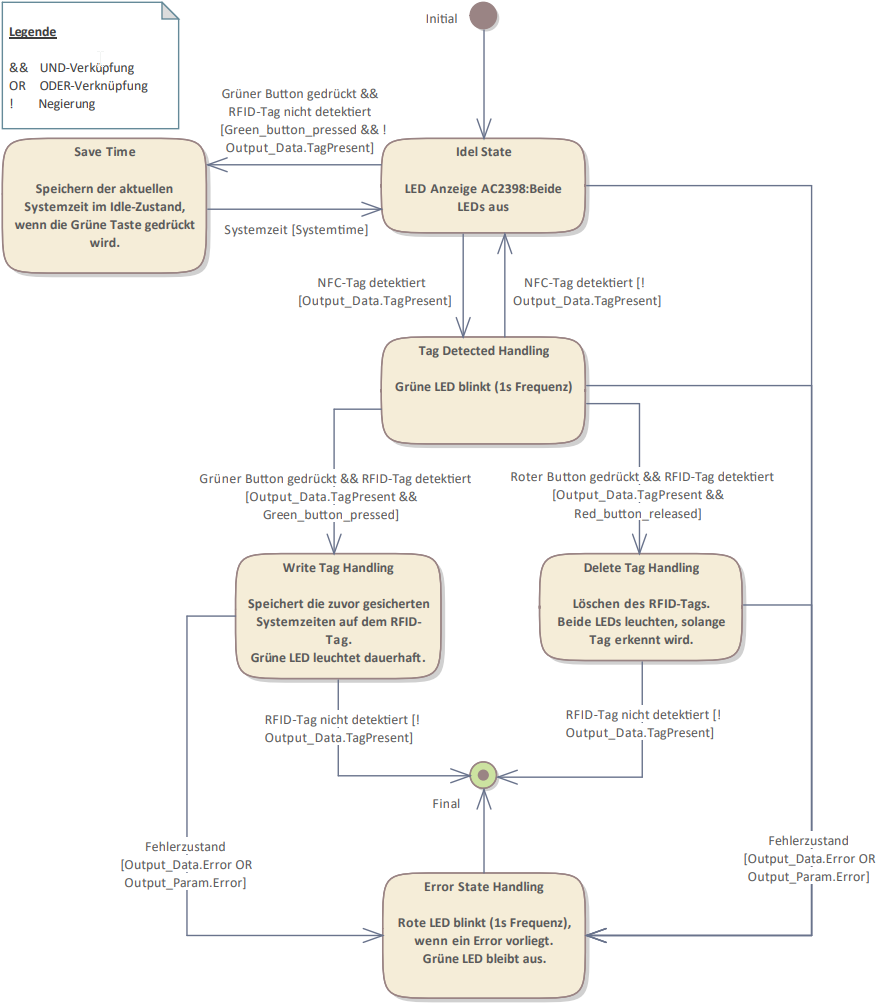
\includegraphics[width=1.0\textwidth]{images/StateMachine.png}
	\caption{State-Machine-Diagramm}
	% [Abbildungsverzeichnis]{Bildunterschrift}
	\label{fig:StateMachineDiagramm}
\end{figure}
% ------------------------------------------------------------------------------------
%... Text Konzeptentwurf: Gegenüberstellung verschiedener Lösungsansätze und Lösungsgenerierung, etc.